% SIAM Article Template
\documentclass[review,onefignum,onetabnum]{siamart171218}

% Information that is shared between the article and the supplement
% (title and author information, macros, packages, etc.) goes into
% ex_shared.tex. If there is no supplement, this file can be included
% directly.


% Packages and macros go here
\usepackage{lipsum}
\usepackage{amsfonts}
\usepackage{graphicx}
\usepackage{epstopdf}
\usepackage{algorithmic}
\ifpdf
  \DeclareGraphicsExtensions{.eps,.pdf,.png,.jpg}
\else
  \DeclareGraphicsExtensions{.eps}
\fi

% Add a serial/Oxford comma by default.
\newcommand{\creflastconjunction}{, and~}

% Used for creating new theorem and remark environments
\newsiamremark{remark}{Remark}
\newsiamremark{hypothesis}{Hypothesis}
\crefname{hypothesis}{Hypothesis}{Hypotheses}
\newsiamthm{claim}{Claim}

% Sets running headers as well as PDF title and authors
\headers{Point Kinetics}{C. Huibregtse}

% Title. If the supplement option is on, then "Supplementary Material"
% is automatically inserted before the title.
\title{Point Kinetics\thanks{Submitted to the editors DATE.}}


% Authors: full names plus addresses.
\author{Clyde Huibregtse\thanks{Massachusetts Institute of Technology Departments of Mathematics and Physics
  (\email{huibregc@mit.edu}, \url{www.google.com}).}}

\usepackage{amsopn}
\DeclareMathOperator{\diag}{diag}

\usepackage{listings}
\lstdefinelanguage{Julia}%
  {morekeywords={struct,abstract,break,case,catch,const,continue,do,else,elseif,%
      end,export,false,for,function,immutable,import,importall,if,in,%
      macro,module,otherwise,quote,return,switch,true,try,type,typealias,%
      using,while},%
   sensitive=true,%
   %alsoother={$},%
   morecomment=[l]\#,%
   morecomment=[n]{\#=}{=\#},%
   morestring=[s]{"}{"},%
   morestring=[m]{'}{'},%
}[keywords,comments,strings]%

\lstset{%
    language         = Julia,
    % basicstyle       = \ttfamily,
    keywordstyle     = \bfseries\color{blue},
    stringstyle      = \color{magenta},
    % commentstyle     = \color{ForestGreen},
    showstringspaces = false,
}


% Optional PDF information
\ifpdf
\hypersetup{
  pdftitle={An Example Article},
  pdfauthor={D. Doe, P. T. Frank, and J. E. Smith}
}
\fi



\begin{document}

\maketitle

% REQUIRED
\begin{abstract}
  This is an example SIAM \LaTeX\ article. This can be used as a
  template for new articles.  Abstracts must be able to stand alone
  and so cannot contain citations to the paper's references,
  equations, etc.  An abstract must consist of a single paragraph and
  be concise. Because of online formatting, abstracts must appear as
  plain as possible. Any equations should be inline.
\end{abstract}

% REQUIRED
\begin{keywords}
  example, \LaTeX
\end{keywords}

% REQUIRED
\begin{AMS}
  68Q25, 68R10, 68U05
\end{AMS}

\section{Point Kinetics and Reactor Dynamics}

\subsection{The Motivation for a Simpler Model}
Reactor dynamics are governed by the transport of energetic neutrons
throughout the active core. In particular, we define the diffusion
of these neutrons in Eq.~\cref{eq:neutron-diffusion}.

\begin{equation}
  \label{eq:neutron-diffusion}
  \frac{\partial N(\vec{r}, t)}{\partial t} = Dv\nabla^2N - \Sigma_a v N + S
\end{equation}

where $N(\vec{r}, t)$ and $S(\vec{r}, t)$ are the neutron density and produced
additional neutron density in some volume $dV$ at location
$\vec{r}$ at time $t$.  $D$ is the diffusion constant; $v$ is the neutron
speed; and $\Sigma_a$ is the macroscopic neutron absorption cross-section. (CITE) \\

Note that this partial differential equation effectively encodes the
conservation of neutrons throughout the core. Neutrons in a given volume of
fuel can: (1) move to an adjacent volume, (2) be absorbed in the given
volume, or (3) be generated as a result of a fission within the volume.\\

This branching structure lends itself wonderfully to the use of
Monte Carlo codes to simulate neutron transport in very high fidelity (CITE SERPENT).
Unfortunately, modeling macroscopic reactor behavior with these high fidelity
tools is infeasible. Coupling the thermalhydraulic behavior of the plant's
power conversion system to the dynamics of subatomic neutrons is
computationally intractable. Consequently, we must create an abstraction from
the neutronics to core-wide dynamics that effectively model important plant
behavior without knowledge of individual neutrons. To do this, we use the
Point Reactor model.

\subsection{The Point Reactor}
The point reactor model operates under a few critical assumptions. First,
it is assumed that the netrons included in $N(\vec{r}, t)$ are all of a single
energy (for our purposes, this is ``fast", rather than ``thermal" energies).
Additionally, our treatment of the neutron production term $S(\vec{r}, t)$
in Eq.~\cref{eq:neutron-diffusion} must be formally defined for the point
reactor. As shown in Eq.~\cref{eq:prompt-delay}, produced neutrons can be of
two types: \emph{prompt} and \emph{delayed}. Prompt neutrons are produced
through direct fission of fuel nuclei, while delayed neutrons are the
byproduct of fission-product decay significantly later than the prompt
generation.

\begin{equation}
  S(\vec{r}, t) = \underbrace{(1-\beta)k_{\infty}\Sigma_avN}_{\text{prompt generation}} + \underbrace{\Sigma_i\lambda_iC_i}_{\text{delay generation}}
  \label{eq:prompt-delay}
\end{equation}

The proportionality constants shown in Eq.~\cref{eq:prompt-delay} are outside
the scope of this analysis. However, $C_i$ refers to the current concentration
of ``delayed neutron group" $i$. It has been shown that the inclusion of six
delayed neutron groups constitutes a reasonably accurate approximation of reactor
dynamics. (CITE FOR NEUTRON GROUPS - Keepin 1965) \\

The final, and most critical assumption the Point Reactor model makes can be
defined as follows: (1) the densities of prompt and delay neutrons are separable
in time and space, and (2) the spatial dependence of prompt neutron density matches
that of delayed neutron density. \\

While the derivation of these final differential equations is outside the scope
of this analysis, they are reproduced in Eqs.~\cref{eq:reac-power,eq:delayed-groups}.

\begin{align}
  \label{eq:reac-power}
  \frac{dn}{dt} &= \frac{\rho - \beta}{\Lambda}n + \Sigma_i\lambda_i c_i \\
  \label{eq:delayed-groups}
  \frac{dc_i}{dt} &= \frac{\beta_i}{\Lambda}n - \lambda_i c_i
\end{align}

Here, formal definition of the parameters is critical to understanding of the
following analysis. Parameters are defined in Eqs.~\Crefrange{eq:param_1}{eq:param_6}.

\begin{align}
  \label{eq:param_1}
  n &= \text{ normalized number of neutrons in the core (effective reactor power)} \\
  \label{eq:param_2}
  c_i &= \text{ normalized number of delayed neutrons of group $i$} \\
  \label{eq:param_3}
  \rho &= \text{ external reactivity (pcm) } \\
  \label{eq:param_4}
  \beta &= \text{ delayed neutron fraction ($\Sigma_i \beta_i$) } \\
  \label{eq:param_5}
  \Lambda &= \text{ mean neutron generation time (s)} \\
  \label{eq:param_6}
  \lambda_i &= \text{ precursor time constants (1/s)}
\end{align}

This ordinary differential equation (ODE) consistutes the primary focus of this
analysis.

\subsection{Important Concepts for this Analysis}
In order to fully understand the process by which we examine this dynamical system,
one must be acquainted with the following terms that are used to describe particular
features of a reactor transient.
\begin{definition}{\textbf{External Reactivity:}}
  External reactivity is defined as an artificial addition (or subtraction) of
  some fraction of the total reactor neutron population. We call any external reacitivity,
  an ``insertion", whether or not it has positive or negative value. It is measured in pcm,
  or per cent mille (0.001\%)
\end{definition}
\begin{definition}{\textbf{Dollar (reactivity):}}
  One dollar of reactivity (\$) is defined as the reactivity required to cross the
  threshold from delayed criticality to prompt criticality. It is numerically equal
  to the $\beta$ constant defined in Eq.~\cref{eq:param_4}.
\end{definition}
\begin{definition}{\textbf{Prompt Criticality:}}
  Prompt criticality refers to a reactor state in which a positive feedback nuclear
  chain reaction is sustained \emph{entirely} by the generation of prompt neutrons.
  This differs from delayed criticality in that it does not require the presense of
  delayed neutron groups to maintain its fission chain reaction. Prompt criticality
  is characterised by fast spikes in power due to the short generation times for
  prompt neutrons.
\end{definition}


\subsection{Analytical Jacobian Analysis}
The form of the ODE defined in Eqs.~\cref{eq:reac-power,eq:delayed-groups},
lead to an analytical definition of this system's Jacobian. (CITE GANOPOL)
Particularly, our system is as defined in Eq.~\cref{eq:dynamical-system}, so
there exists a true form of the Jacobian, shown in Eq.~\cref{eq:jacobian-definition}.

\begin{align}
  \label{eq:dynamical-system}
  \frac{du}{dt} &= A(t)u\\
  \label{eq:jacobian-definition}
  A(t) &= \begin{pmatrix}\frac{\rho(t)-\beta}{\Lambda}&\lambda_1&\lambda_2&\cdots&\lambda_6\\
                      \frac{\beta_1}{\Lambda}&-\lambda_1&0&\cdots&0\\
                      \frac{\beta_2}{\Lambda}&0&-\lambda_2&\cdots&0\\
                      \vdots&\vdots&\vdots&\ddots&\vdots\\
                      \frac{\beta_6}{\Lambda}&0&0&\cdots&-\lambda_6\end{pmatrix}
\end{align}

Here, $A(t)$ is the time dependent Jacobian for our dynamical system. Note the
time independence for all but the prompt neutron term. This is a critical feature
of the system. We can see that, at operating conditions where $0 \leq \rho(t) < \beta = 1\$$,
all of the diagonal terms of our Jacobian are negative. This property ensures
that the reactor is in a delayed critical state, and the unbounded growth in power
is relatively slow. Transients in which $\rho(t) \geq \beta = 1\$$ have Jacobians with
a positive diagonal element. This corresponds to the reactor going prompt critical, and
the reactor power grows without bound millions of times faster than when it is delayed
critical. \\

There are a few things to note: (1) the unbounded growth of reactor power seen
in transients with positive $\rho(t)$ parameters is a numerical phenomenon. In reality,
nuclear material undergoes a ``fizzle" (CITE) that limits this rapid overpower (except
in the cases of nuclear weapons). This effect is not captured in the Point Reactor
model, but does not affect solutions around the time of reacitivity insertion. (2) For
sections of a reactor transient timeseries over which $\rho(t)$ is constant, there is an
analytical solution to the dynamical system involving a series of exponential functions
defined by the eigenvalues of $A$. \\

For the purposes of building a modeling tool that can aid in iterating reactor design,
we focus our analysis on the efficacy of solver methods on the order of $100 pcm$
reactivity insertions. These insertions correspond to moderate transients seen during
normal operations. To be exhaustive, however, we will also examine the efficacy of our
solver algorithms under a $1$\$ insertion. While it is more an exercise in academia than
practical engineering, an understanding of large insertions may give insight into the
rubustness of these solution  algorithms.

\subsection{The Analytical Solution to the Step Insertion}
As previously stated, in cases where $\rho(t)$ is constant, there exists an
analytical solution to the point kinetics ODE. The  This solution is reproduced in
Eq.~\cref{eq:analytical-step}.

\begin{align}
  \label{eq:analytical-step}
  \Psi &= \Sigma_{k=0}^K \left( (-1)^k \Sigma_{j=0}^K \left( \frac{e^{\omega_jt}B_{K-k,j}}{\Pi_{i=0, i\neq j}^K (\omega_i - \omega_j)}\right) A^k\right)\Psi_0\\
  \text{where } B_{m,n} &= \Sigma_{i_1 = 1, i_1 \neq j}^K \Sigma_{i_2 = i_1 + 1, i_2 \neq j}^K ...\Sigma_{i_m = i_{m-1} + 1, i_m \neq j}^K \omega_{i_1}\omega_{i_2}...\omega_{i_m}
\end{align}
(CITE SOLUTION)
Each $\omega_i$ is an eigenvalue of the Jacobian $A$, or is a root of the inhour
equation:

\begin{equation}
  \rho = \Lambda\omega + \omega \Sigma_{k=1}^K \frac{\beta_k}{\omega + \lambda_k}
\end{equation}

Note that the formal definition fo this analytical solution has, in the denominator
of each summed term, a large product of eigenvalue differences. This procedure of
multiplying a sequence of differences is reminiscent of the Lagrange basis polynomial
definition, where our dataset is the set of eigenvalues of $A$. Consequently,
we encounter some numerical instability when evaluating this analytical solution.
Figure~\cref{fig:single-double-prec} shows how we avoid this floating point
imprecision by making use of the \texttt{DoubleFloats.jl} package.\\

\begin{figure}[htb]
  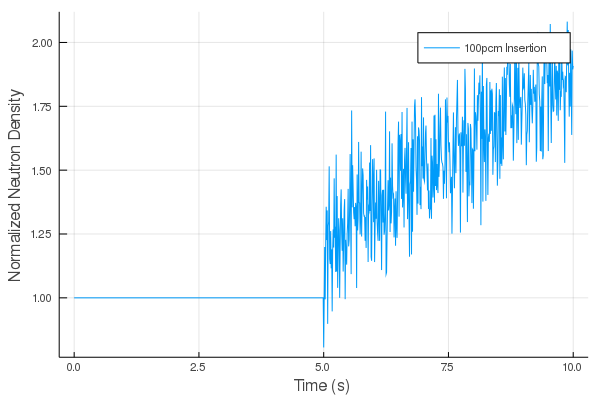
\includegraphics[width=0.5\textwidth]{../plots/analytical-sols/100pcm_fp_error.png}
  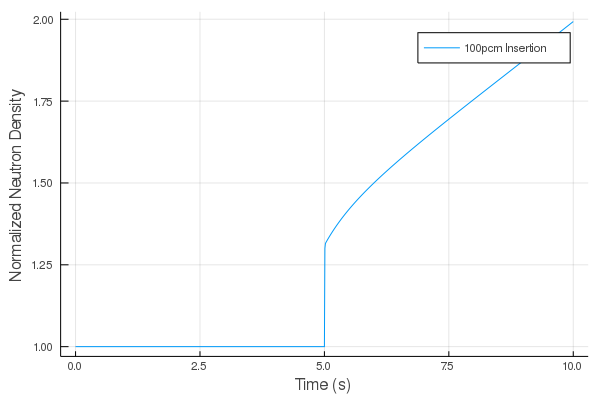
\includegraphics[width=0.5\textwidth]{../plots/analytical-sols/100pcm.png}
  \caption{Left: The analytical solution to the Point Kinetics equations under a $100$ pcm insertion
  as defined in Eq.~\cref{eq:analytical-step} with use of the native \texttt{Float64} precision.
  Right: The same solution, but instead with \texttt{Double64} (a $128$ bit floating point number)
  as the basis. The error is resolved, and the pertinent features are evident. The insertions occur
  at $t = 5$s.}
  \label{fig:single-double-prec}
\end{figure}

Additionally, we will examine reactivity insertions on the order of $1$\$, which
diverge very quickly. Figure~\cref{fig:dollar-insert-analytical} shows the analytical
solution to the point kinetics equations under a step insertion of $1$\$.

\begin{figure}[htb]
  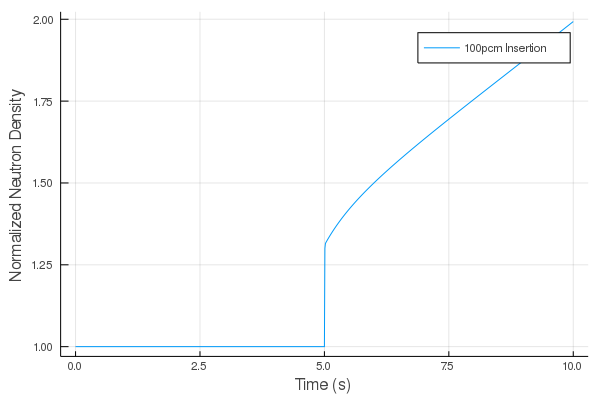
\includegraphics[width=0.5\textwidth]{../plots/analytical-sols/100pcm.png}
  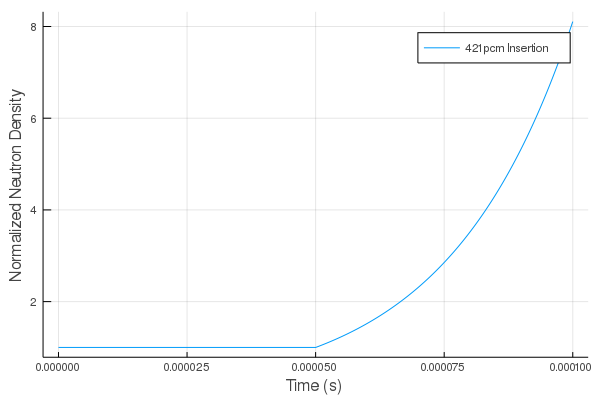
\includegraphics[width=0.5\textwidth]{../plots/analytical-sols/421pcm.png}
  \caption{Left: A reproduction of the right plot from Figure~\cref{fig:single-double-prec}.
  Right: The analytical solution defined in Eq.~\cref{eq:analytical-step} with a
  reactivity insertion of $1$\$ or $421$ pcm. Note that the prompt jump is so large that the
  solution diverges within a thousandth of a second. These two curves represent our
  test case solutions.}
  \label{fig:dollar-insert-analytical}
\end{figure}

These two curves are a baseline to which we compare all of our computed solutions,
giving a quantifiable metric for accuracy in both tranients.

\section{Solving the Point Kinetics Equations}

\subsection{Building an Optimal Derivative Defintion}
In order to perform any sort of reasonable benchmarking for solver algorithms,
we must ensure that our ODE definition is optimal, such that any discrepancies in
solution time are not drowned out by overhead. There are a few things we can check
to ensure optimality in our ODE definition: (1) memory allocations, (2) type stability,
and (3) solver overhead. \\

Using the \texttt{BenchmarkTools.jl} \texttt{@btime} and \texttt{@benchmark} macros,
we can demonstrate that our inner loop (the \texttt{pk!} method) has minimal allocations.
Particularly, we can achieve almost no (2) heap allocations per inner loop (a result of
our two \texttt{@view} macro calls), totalling only $96$ bytes. \\

Now we can use the type inferencing capabilities of \texttt{Julia}'s JIT compiler
to speed up our solves. To achieve type stability, we define an abstract type family,
\texttt{AbstractInsert}, that handles arbitraty reactivity insertion functions.
This allows the parameters used within the inner loop to be fully type stable.
The \texttt{@code\_warntype} macro shows no potential type
ambiguities throughout our inner loop, so we can be assured the JIT compiler is
producing optimal type inferences. \\

Finally, we can use the \texttt{Profle.jl} module to corroborate the above two
conclusions, that, our ODE definition is in fact optimal. This
plot shows the relative time spent in each function called during the solve. Highlighted
in Figure~\cref{fig:flame-plot} are sections of importance. In general, though,
there is little overhead from the solver, so most of the computation time is spent
doing the actual integration.\\

\begin{figure}[htb]
  % \includegraphics[width=0.5\textwidth]{../plots/flame-plots/100pcm_flame_plot.png}
  \caption{}
  \label{fig:flame-plot}
\end{figure}

Now we can effectively dive into a solver analysis with the guarantee that algorithmic
differences in the integrators produce the variance in the total runtimes, and not
computational inefficiencies.

\subsection{Metrics for Evaluating Integrator Performance}
In the following sections we present a detailed analysis of the efficacy of a litany of solvers
at a variety of tolerances. The best metric for rating the performace of a solver algorithm
is an open question. The best choice is user-specific, so for the sake of making a
conclusion, we specify our user needs here. We set out to create a high-speed,
reasonably accurate simulator to be used in core design work and reactor control
optimizations. There are a few key threshold criteria that we require of our simulator:\\

\begin{enumerate}
  \item Resolve the prompt jump to very high fidelity ($10^{-6}$ or better)
  \item Approximate netron densities during delayed effects to an accuracy within $10^-4$
  \item Have the ability to accept a reactivity insertion of arbitrary shape
  \item Outperform an existing Python implementation.
\end{enumerate}







% % The outline is not required, but we show an example here.
% The paper is organized as follows. Our main results are in
% \cref{sec:main}, our new algorithm is in \cref{sec:alg}, experimental
% results are in \cref{sec:experiments}, and the conclusions follow in
% \cref{sec:conclusions}.
%
% \section{Main results}
% \label{sec:main}
%
% We interleave text filler with some example theorems and theorem-like
% items.
%
% \lipsum[4]
%
% Here we state our main result as \cref{thm:bigthm}; the proof is
% deferred to \cref{sec:proof}.
%
% \begin{theorem}[$LDL^T$ Factorization \cite{GoVa13}]\label{thm:bigthm}
%   If $A \in \mathbb{R}^{n \times n}$ is symmetric and the principal
%   submatrix $A(1:k,1:k)$ is nonsingular for $k=1:n-1$, then there
%   exists a unit lower triangular matrix $L$ and a diagonal matrix
%   \begin{displaymath}
%     D = \diag(d_1,\dots,d_n)
%   \end{displaymath}
%   such that $A=LDL^T$. The factorization is unique.
% \end{theorem}
%
% \lipsum[6]
%
% \begin{theorem}[Mean Value Theorem]\label{thm:mvt}
%   Suppose $f$ is a function that is continuous on the closed interval
%   $[a,b]$.  and differentiable on the open interval $(a,b)$.
%   Then there exists a number $c$ such that $a < c < b$ and
%   \begin{displaymath}
%     f'(c) = \frac{f(b)-f(a)}{b-a}.
%   \end{displaymath}
%   In other words,
%   \begin{displaymath}
%     f(b)-f(a) = f'(c)(b-a).
%   \end{displaymath}
% \end{theorem}
%
% Observe that \cref{thm:bigthm,thm:mvt,cor:a} correctly mix references
% to multiple labels.
%
% \begin{corollary}\label{cor:a}
%   Let $f(x)$ be continuous and differentiable everywhere. If $f(x)$
%   has at least two roots, then $f'(x)$ must have at least one root.
% \end{corollary}
% \begin{proof}
%   Let $a$ and $b$ be two distinct roots of $f$.
%   By \cref{thm:mvt}, there exists a number $c$ such that
%   \begin{displaymath}
%     f'(c) = \frac{f(b)-f(a)}{b-a} = \frac{0-0}{b-a} = 0.
%   \end{displaymath}
% \end{proof}
%
% Note that it may require two \LaTeX\ compilations for the proof marks
% to show.
%
% Display matrices can be rendered using environments from \texttt{amsmath}:
% \begin{equation}\label{eq:matrices}
% S=\begin{bmatrix}1&0\\0&0\end{bmatrix}
% \quad\text{and}\quad
% C=\begin{pmatrix}1&1&0\\1&1&0\\0&0&0\end{pmatrix}.
% \end{equation}
% Equation \cref{eq:matrices} shows some example matrices.
%
% We calculate the Fr\'{e}chet derivative of $F$ as follows:
% \begin{subequations}
% \begin{align}
%   F'(U,V)(H,K)
%   &= \langle R(U,V),H\Sigma V^{T} + U\Sigma K^{T} -
%   P(H\Sigma V^{T} + U\Sigma K^{T})\rangle \label{eq:aa} \\
%   &= \langle R(U,V),H\Sigma V^{T} + U\Sigma K^{T}\rangle
%   \nonumber \\
%   &= \langle R(U,V)V\Sigma^{T},H\rangle +
%   \langle \Sigma^{T}U^{T}R(U,V),K^{T}\rangle. \label{eq:bb}
% \end{align}
% \end{subequations}
% % \Cref{eq:aa} is the first line, and \cref{eq:bb} is the last line.
%
% \section{Algorithm}
% \label{sec:alg}
%
% \lipsum[40]
%
% Our analysis leads to the algorithm in \cref{alg:buildtree}.
%
% \begin{algorithm}
% \caption{Build tree}
% \label{alg:buildtree}
% \begin{algorithmic}
% \STATE{Define $P:=T:=\{ \{1\},\ldots,\{d\}$\}}
% \WHILE{$\#P > 1$}
% \STATE{Choose $C^\prime\in\mathcal{C}_p(P)$ with $C^\prime := \operatorname{argmin}_{C\in\mathcal{C}_p(P)} \varrho(C)$}
% \STATE{Find an optimal partition tree $T_{C^\prime}$ }
% \STATE{Update $P := (P{\setminus} C^\prime) \cup \{ \bigcup_{t\in C^\prime} t \}$}
% \STATE{Update $T := T \cup \{ \bigcup_{t\in\tau} t : \tau\in T_{C^\prime}{\setminus} \mathcal{L}(T_{C^\prime})\}$}
% \ENDWHILE
% \RETURN $T$
% \end{algorithmic}
% \end{algorithm}
%
% \lipsum[41]
%
% \section{Experimental results}
% \label{sec:experiments}
%
% \lipsum[50]
%
% % \Cref{fig:testfig} shows some example results. Additional results are
% % available in the supplement in \cref{tab:foo}.
%
% \begin{figure}[htbp]
%   \centering
%   % \label{fig:a}\includegraphics{lexample_fig1}
%   \caption{Example figure using external image files.}
%   \label{fig:testfig}
% \end{figure}
%
% \lipsum[51]
%
% \section{Discussion of \texorpdfstring{{\boldmath$Z=X \cup Y$}}{Z = X union Y}}
%
% \lipsum[76]
%
% \section{Conclusions}
% \label{sec:conclusions}
%
% Some conclusions here.
%

\appendix
\section{An example appendix}


\begin{lemma}
Test Lemma.
\end{lemma}


\section*{Acknowledgments}
We would like to acknowledge the assistance of volunteers in putting
together this example manuscript and supplement.

\bibliographystyle{siamplain}
\bibliography{references}
\end{document}
